\documentclass[tikz,border=1mm]{standalone}
\usepackage{tikz, mathrsfs, amssymb, mathtools}

\definecolor{vivamagenta}{RGB}{190,52,85}
\definecolor{azul}{RGB}{142,125,190}

\begin{document}

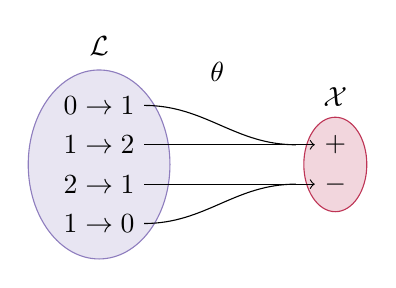
\begin{tikzpicture}
        % draw the sets
        \filldraw[fill=azul!20, draw=azul!100] (-1.5,.5) ellipse (.9cm and 1.2cm);
        \filldraw[fill=vivamagenta!20, draw=vivamagenta!100] (1.5,.5) ellipse (0.4cm and .6cm);
    
        % names
        \node at (1.5,1.35) {$\mathcal{X}$};
        \node at (0, 1.675) {$\theta$};
        \node at (-1.5,2) {$\mathcal{L}$};
    
        % mathbb L
        \node (y1) at (1.5,0.75) {$+$};
        \node (y2) at (1.5,0.25) {$-$};

        % L
        \node (x1) at (-1.5,1.25) {$0 \to 1$};
        \node (x2) at (-1.5,0.75) {$1 \to 2$};
        \node (x3) at (-1.5,0.25) {$2 \to 1$};
        \node (x4) at (-1.5,-0.25) {$1 \to 0$};

        % map
        \path (x1) edge [out=0, in=180] (1,0.75);
        \path (x2) edge [out=0, in=180] (1,0.75);
        \draw[->] (1,0.75) -- (y1);
        \path (x3) edge [out=0, in=180] (1,0.25);
        \path (x4) edge [out=0, in=180] (1,0.25);
        \draw[->] (1,0.25) -- (y2);
        
    \end{tikzpicture}

\end{document}
